%%%%%%%%%%%%%%%%%%%%%%%%%%%%%%%%%%%%%%%%%
% Wenneker Article
% LaTeX Template
% Version 2.0 (28/2/17)
%
% This template was downloaded from:
% http://www.LaTeXTemplates.com
%
% Authors:
% Vel (vel@LaTeXTemplates.com)
% Frits Wenneker
%
% License:
% CC BY-NC-SA 3.0 (http://creativecommons.org/licenses/by-nc-sa/3.0/)
%
%%%%%%%%%%%%%%%%%%%%%%%%%%%%%%%%%%%%%%%%%

%----------------------------------------------------------------------------------------
%	PACKAGES AND OTHER DOCUMENT CONFIGURATIONS
%----------------------------------------------------------------------------------------

\documentclass[10pt, a4paper, twocolumn]{article} % 10pt font size (11 and 12 also possible), A4 paper (letterpaper for US letter) and two column layout (remove for one column)

%%%%%%%%%%%%%%%%%%%%%%%%%%%%%%%%%%%%%%%%%
% Wenneker Article
% Structure Specification File
% Version 1.0 (28/2/17)
%
% This file originates from:
% http://www.LaTeXTemplates.com
%
% Authors:
% Frits Wenneker
% Vel (vel@LaTeXTemplates.com)
%
% License:
% CC BY-NC-SA 3.0 (http://creativecommons.org/licenses/by-nc-sa/3.0/)
%
%%%%%%%%%%%%%%%%%%%%%%%%%%%%%%%%%%%%%%%%%

%----------------------------------------------------------------------------------------
%	PACKAGES AND OTHER DOCUMENT CONFIGURATIONS
%----------------------------------------------------------------------------------------

\usepackage[english]{babel} % English language hyphenation

\usepackage{microtype} % Better typography

\usepackage{amsmath,amsfonts,amsthm} % Math packages for equations

\usepackage[svgnames]{xcolor} % Enabling colors by their 'svgnames'

\usepackage[hang, small, labelfont=bf, up, textfont=it]{caption} % Custom captions under/above tables and figures

\usepackage{booktabs} % Horizontal rules in tables

\usepackage{lastpage} % Used to determine the number of pages in the document (for "Page X of Total")

\usepackage{graphicx} % Required for adding images

\usepackage{enumitem} % Required for customising lists
\setlist{noitemsep} % Remove spacing between bullet/numbered list elements

\usepackage{sectsty} % Enables custom section titles
\allsectionsfont{\usefont{OT1}{phv}{b}{n}} % Change the font of all section commands (Helvetica)

%----------------------------------------------------------------------------------------
%	MARGINS AND SPACING
%----------------------------------------------------------------------------------------

\usepackage{geometry} % Required for adjusting page dimensions

\geometry{
	top=1cm, % Top margin
	bottom=1.5cm, % Bottom margin
	left=2cm, % Left margin
	right=2cm, % Right margin
	includehead, % Include space for a header
	includefoot, % Include space for a footer
	%showframe, % Uncomment to show how the type block is set on the page
}

\setlength{\columnsep}{7mm} % Column separation width

%----------------------------------------------------------------------------------------
%	FONTS
%----------------------------------------------------------------------------------------

\usepackage[T1]{fontenc} % Output font encoding for international characters
\usepackage[utf8]{inputenc} % Required for inputting international characters

\usepackage{XCharter} % Use the XCharter font

%----------------------------------------------------------------------------------------
%	HEADERS AND FOOTERS
%----------------------------------------------------------------------------------------

\usepackage{fancyhdr} % Needed to define custom headers/footers
\pagestyle{fancy} % Enables the custom headers/footers

\renewcommand{\headrulewidth}{0.0pt} % No header rule
\renewcommand{\footrulewidth}{0.4pt} % Thin footer rule

\renewcommand{\sectionmark}[1]{\markboth{#1}{}} % Removes the section number from the header when \leftmark is used

%\nouppercase\leftmark % Add this to one of the lines below if you want a section title in the header/footer

% Headers
\lhead{} % Left header
\chead{\textit{\thetitle}} % Center header - currently printing the article title
\rhead{} % Right header

% Footers
\lfoot{} % Left footer
\cfoot{} % Center footer
\rfoot{\footnotesize Page \thepage\ of \pageref{LastPage}} % Right footer, "Page 1 of 2"

\fancypagestyle{firstpage}{ % Page style for the first page with the title
	\fancyhf{}
	\renewcommand{\footrulewidth}{0pt} % Suppress footer rule
}

%----------------------------------------------------------------------------------------
%	TITLE SECTION
%----------------------------------------------------------------------------------------

\newcommand{\authorstyle}[1]{{\large\usefont{OT1}{phv}{b}{n}\color{DarkRed}#1}} % Authors style (Helvetica)

\newcommand{\institution}[1]{{\footnotesize\usefont{OT1}{phv}{m}{sl}\color{Black}#1}} % Institutions style (Helvetica)

\usepackage{titling} % Allows custom title configuration

\newcommand{\HorRule}{\color{DarkGoldenrod}\rule{\linewidth}{1pt}} % Defines the gold horizontal rule around the title

\pretitle{
	\vspace{-30pt} % Move the entire title section up
	\HorRule\vspace{10pt} % Horizontal rule before the title
	\fontsize{32}{36}\usefont{OT1}{phv}{b}{n}\selectfont % Helvetica
	\color{DarkRed} % Text colour for the title and author(s)
}

\posttitle{\par\vskip 15pt} % Whitespace under the title

\preauthor{} % Anything that will appear before \author is printed

\postauthor{ % Anything that will appear after \author is printed
	\vspace{10pt} % Space before the rule
	\par\HorRule % Horizontal rule after the title
	\vspace{20pt} % Space after the title section
}

%----------------------------------------------------------------------------------------
%	ABSTRACT
%----------------------------------------------------------------------------------------

\usepackage{lettrine} % Package to accentuate the first letter of the text (lettrine)
\usepackage{fix-cm}	% Fixes the height of the lettrine

\newcommand{\initial}[1]{ % Defines the command and style for the lettrine
	\lettrine[lines=3,findent=4pt,nindent=0pt]{% Lettrine takes up 3 lines, the text to the right of it is indented 4pt and further indenting of lines 2+ is stopped
		\color{DarkGoldenrod}% Lettrine colour
		{#1}% The letter
	}{}%
}

\usepackage{xstring} % Required for string manipulation

\newcommand{\lettrineabstract}[1]{
	\StrLeft{#1}{1}[\firstletter] % Capture the first letter of the abstract for the lettrine
	\initial{\firstletter}\textbf{\StrGobbleLeft{#1}{1}} % Print the abstract with the first letter as a lettrine and the rest in bold
}

%----------------------------------------------------------------------------------------
%	BIBLIOGRAPHY
%----------------------------------------------------------------------------------------

\usepackage[backend=bibtex,style=numeric,natbib=true,sorting=none]{biblatex} % Use the bibtex backend with the authoryear citation style (which resembles APA)

\addbibresource{bib/citation-316688593.bib} % The filename of the bibliography
\addbibresource{bib/ILCPA.64.159.bib}
\addbibresource{bib/ScienceDirect_citations_1670195837352.bib}
\addbibresource{bib/misc.bib}

\usepackage[autostyle=true]{csquotes} % Required to generate language-dependent quotes in the bibliography
 % Specifies the document structure and loads requires packages

\usepackage{wrapfig}
\usepackage{hyperref}

%----------------------------------------------------------------------------------------
%	ARTICLE INFORMATION
%----------------------------------------------------------------------------------------

\title{Nonlinear Wave Propagation Effects in Optical Fibers} % The article title

\author{
	\authorstyle{Nathan Constantinides\textsuperscript{1}}% Authors
	\newline\newline % Space before institutions
	\textsuperscript{1}\institution{University of Maryland, College Park}\\ % Institution 1
}

% Example of a one line author/institution relationship
%\author{\newauthor{John Marston} \newinstitution{Universidad Nacional Autónoma de México, Mexico City, Mexico}}

\date{December 18, 2022} % Add a date here if you would like one to appear underneath the title block, use \today for the current date, leave empty for no date

%----------------------------------------------------------------------------------------
\begin{document}

\maketitle % Print the title

\thispagestyle{firstpage} % Apply the page style for the first page (no headers and footers)

%----------------------------------------------------------------------------------------
%	ABSTRACT
%----------------------------------------------------------------------------------------

% \lettrineabstract{}

%----------------------------------------------------------------------------------------
%	ARTICLE CONTENTS
%----------------------------------------------------------------------------------------

% \setcitestyle{numbers}

\section{Overview of Non-Linear Optics}
Optical fibers form pathways by which the transmission of high frequency (often infrared to visible) electro-magnetic waves can be directed over relatively long distances with high signal fidelity. Optical fibers are typically formed by a high refractive index glass core, surrounded by a less refractive cladding layer, all wrapped by one final layer of an even lower refractive index jacket \cite{AgrawalChap1}. This structure forces light that has entered the fiber to propagate along its core through the principles of Snell's law, as the changes in refractive index between the core and the cladding ensure that the cable causes total internal reflection, as well as that a very low amount of it escapes the medium to the external environment. One might be tempted to treat an optical fiber as a perfect vacuum that does not impact signal quality; after all, this would be the ideal context for high speed communication with optical wave packets. In practice, however, fibers far from ensure perfect signal coherence; their performance exhibits a combination of loss due to photon scattering, absorption, and chromatic and polarization dispersion, alongside a plethora of other phenomenon that generally do not play significant roles in silica fibers but are certainly important to the broader field of non-linear optics \cite{AgrawalChap1}. All of these factors impose fundamental limits on information transfer, and with the increasing demands of internet infrastructure, interest in understanding and mitigating these effects has piqued, especially following the 1990s. 

This paper will explore a the simulation of a model of pulse propagation that takes into account the important non-linear optical effects of chromatic dispersion and self phase modulation. This model is formed by a characteristic "Nonlinear Schrodinger Equation" that may be simulated through a method of fourier analysis referred to as the "Split Step Fourier Method".

\section{Non-Linear Effects in Optical Fibers}

\subsection{Loss}
The simplest effect that one can consider in an optical fiber wave guide is that of signal strength loss. As electromagnetic waves travel in the fiber, their energy is dissipated into the medium through two main processes known as "material absorption" and "Rayleigh scattering". Material absorption is a process that is intutively familiar, and is caused by the presence of fiber defects and impurities, as well as the effect that photons travelling through the silica medium excite the resonances of electrons orbiting silica nuclei, thus dissipating the lights energy \cite{AgrawalChap1}. Due to the natural frequencies of these electronic resonances, silica fibers are known to also display lower amounts of loss in certain wavelength ranges, which generally fall within 0.5 to 2 $\mu m$ \cite{AgrawalChap1}. 

While material absorption is simply fundamental to the behavior of silica atoms, Rayleigh scattering is a process that is much more dependent on the manufacturing quality of an optical fiber. During the fabrication process, fluctuations in the density of the silica core can cause the refractive properties of the cable to change at different positions in the medium. The changes due to both material absorption and Rayleigh scattering are accounted for with the experimental determination of the attenuation constant, $\alpha$, of each fiber. This constant is approximated to change the power of electromagnetic waves in a medium by 
$$P_T = P_0 e^{-\alpha L}$$
where $P_0$ is initial pulse power, and $P_T$ is the pulse power after a pulse has travelled a distance $L$ in the fiber.

\subsection{Chromatic Dispersion}
Another important, non-linear effect observable in optical fibers is that of chromatic dispersion, the process by which the refractive index obtains a frequency dependence $n(w)$. The effect is derivative of the fact that the interaction of electromagnetic waves with a dielectric causes bound electrons in the material to oscillate at certain resonant frequencies, causing differences in responses of the medium to waves with different frequencies. The refractive index for such a dispersive medium is described by the Sellmeier equation \cite{AgrawalChap2}:
$$n^2(\omega) = \sum_{j=1}^m \frac{B_j \omega_j^2}{\omega_j^2 - \omega^2}$$
Here, each $\omega_j$ and $B_j$ correspond to a resonance and its strength, respectively. These values are determined experimentally, and when doing so may be expressed in terms of $\lambda_j$ and related via 
$$\lambda_j = 2\pi c \omega_j$$
For convience, the refractive index is often related to a taylor series for a new value $\beta(\omega)$
\begin{align*}
    \beta (\omega) = \frac{n(\omega)\cdot\omega}{c} = \beta_0 + \beta_1 (\omega - \omega_0) +\\ \frac{1}{2} \beta_2 (\omega - \omega_0)^2 + \frac{1}{6} \beta_3 (\omega - \omega_0)^3...
\end{align*}
Each $\beta_m$ is simply short-hand for $\frac{d^m\beta}{d\omega ^m}$, and can also be determined via experiment. $\beta$ is sometimes called the "Wave Propagation Constant" and takes the place of $k$ in the familar $A e^{kx - \omega t}$ equation for a wave with a singular frequency. As I will demonstrate soon, we will only consider the effects up to the $\beta_2$ dispersive parameter for the sake of simplicity and so that an approximate model of pulse propagation can be simulated.

\subsection{Induced Polarization and the Optical Kerr Effect}
The final significant nonlinear optical effect that we will consider in our investigation of waves in silica fibers is that of the Optical Kerr Effect. After entering a dielectric, electromagnetic waves may induce changes in the motion of bound electrons (similar to driven oscillation), and in turn make changes to their resonant frequencies and their influence on the refractive index of the medium. This intensity dependent change in the refractive index is observed more generally in other mediums for electromagnetic waves, and is responsible for the fascinating effects of self phase modulation and self induced phase and frequency shifting (or chirping) observed in silica fibers. More generally, it also can cause self-focusing of beams of light in space, however this is not observed in optical fibers due to the spatial constrictions they place on light entering the medium. The effect of the Kerr effect is usually assumed to take the following form:
$\tilde{n}(I) = n(w) + n_2 I$, where $I$ is proportional to the squared magnitude of the electric field $|E|^2$ \cite{AgrawalChap1}

% \subsection{Group Velocity Dispersion}
% Now that we understand the process of chromatic dispersion in optical fibers, we can inspect that of group velocity dispersion. Looking back at our relation for chromatic dispersion, one should note that the group velocity of the system is not constant with respect to $\omega$, therefore it is expected that the optical medium exhibits group velocity dispersion, where different wave lengths of light travel at fundamentally different frequencies than others. 

% \subsection{Solitons}

\section{The Non-Linear Schrodinger Equation}
It is shown in Agrawal that there exists a characteristic equation for the evolution of pulses in optical fibers. This equation is referred to as the "Nonlinear Schrodinger Equation" and is written as follows \cite{AgrawalChap2}:
$$\frac{\partial A}{\partial z} + \beta_1 \frac{\partial A}{\partial t} i\frac{\beta_2}{2}\frac{\partial^2 A}{\partial t^2} + \frac{\alpha}{2} = i \gamma(\omega_0)|A|^2A$$
This equation introduces several important parameters that we need to consider in our wave propagation model. Firstly, the $A$ term is the complex-valued amplitude of the group velocity wave envelope that surrounds the electromagnetic wave in a dispersive medium. $\beta_1$ and $\beta_2$ are the familiar constants from the taylor expansion of the wave propagation constant $\beta$ induced by chromatic dispersion, and $\alpha$ is the already established "attenuation" constant that governs the effects of fiber losses. The last unfamiliar term is the $\gamma(\omega_0)$ constant. $\gamma$ is referred to as the "nonlinearity parameter" and is repsonsible for introducing the effects of the intensity dependence of the fiber medium on the wave. This equation does not consider chromatic dispersion terms above $\beta_2$ for the reason that it expects to be used to model pulses of width on the order of ~$10\ ps$, in which Agrawal shows that these higher order terms have negligible impact on the propagation of the wave.

It should be noted that $A$ is normalized by some scalar so that $|A|^2$ will have units of Watts and be equivalent to the intensity of the optical pulse. The term $\omega_0$ is also the expected "carrier frequency" of the pulse, or the frequency at which the pulse spectrum is centered, thus this model only takes into account the effect of medium nonlinearity in a narrow range surrounding one's chosen $\omega_0$.

\section{Effects on Pulse Propagation}

\subsection{Group Velocity Dispersion / Pulse Broadening}
Using this model of pulse propagation, we can create an approximate, but useful demonstration of an electromagnetic pulse that travels in an optical fiber. The first effect that we wish to see in our demonstration will be that of group velocity dispersion. If we ignore all the effects on the system except that of chromatic dispersion, we get a simplified relation
$$\frac{\partial A}{\partial Z} = \frac{i\beta_2}{2} \frac{\partial^2 A}{\partial T^2}$$
Where $T$ is a moving time reference frame that follows the center of the pulse group velocity as it travels along the fiber, with $T = t - z/v_g$. This is equaivalent to setting the parameters $\gamma$ and $\alpha$ to zero. Given an initial pulse shape, $A(0, T)$, this equation may be solved with a fourier transform \cite{AgrawalChap3}:
$$U(z, t) = \mathbb{F}^{-1} \left\{ \mathbb{F} \{A(0, T)\} e^{\frac{i}{2} \beta_2 \omega^2 z} \right\}$$
If the initial pulse is guassian shape, with full width at half maximum (FWHM) $2(\ln 2 )^{1/2} T_0$, then we have:
$$A(0, T) = e^{-\frac{T^2}{2t_0^2}}$$
And if we substitute this into this solution format we obtain \cite{AgrawalChap3}: 
$$A(z, T) = \frac{T_0}{T_0^2 - i\beta_2 z}^{1/2} e^{\frac{-T^2}{2(T_0^2 - i \beta_2 z)}}$$
This expression reveals that as the pulse propagates over Z, not only does its amplitude coefficent decrease proportionally to $1/\sqrt{z}$, it's FWHM also increases proportionally to $\sqrt{z}$. This is the pulse broadening or group velocity dispersion effect, and we will explore it in a simulation shortly.

\subsection{Self Phase Modulation}
When we found a solution for a system that only employs group velocity dispersion, we neglected the non-linear effects of self phase modulation. It is worth mentioning at this point, that there exists a method by which to gauge the importance of group velocity dispersion versus self phase modulation. The non-linearity parameter \cite{AgrawalChap3}
$$N = \left(\frac{\gamma P_0 T_0^2}{\vert \beta_2 \vert}\right)^{\frac{1}{2}}$$
is a dimensionless value, with $T_0$ as the familiar guassian spread parameter and $P_0$ is the input pulse's peak power. If $N >> 1$, the effects of self phase modulation will become dominant in the system, and in the case $N << 1$ dispersion is the dominant non-linear effect (hence why $\gamma = 0$ eliminated the effects of self phase modulation in the prior section)\cite{AgrawalChap3}. The effect of having a high $N$, and thus significant self phase modulation, is that there will be a spectral broadening of guassian pulses in the fiber medium, and an increase in chirp ("chirping") as one follows the the length of the fiber.

\section{Simulation}

\subsection{Split Step Fourier Method}
When looking to implement a simulation of the pulse behavior, the first (and most accurate) methodology one should consider is the splt step fourier method. Other less computationally expensive methods (such as some finite difference methods) exist and might work better for simulations of very long range fibers, but in general the split step method is preferred.

For the equation for the pulse envelope $A$, there is a way to decompose the partial differential equation into two operators, such that we can write it in the form:
$$\frac{\partial A}{\partial z} = (\hat{D} + \hat{N})A$$
The $\hat{D}$ operator will represent the linear effects of the system on $A$, and the $\hat{N}$ operator will represent the non-linear effects of the system on $A$. For the more general equation for $A$ that takes into account the third order chromatic dispersion and Raman Scattering, the operators $D$ and $N$ are: \cite{Munaweera}:
\begin{align*}
    \hat{D} &= \frac{-i\beta_2}{2} \frac{\partial^2}{\partial T^2} + \frac{\beta_3}{6}\frac{\partial^3}{\partial T^3} - \frac{\alpha}{2}\\
    \hat{N} &= i\gamma \left(|A|^2 + \frac{i}{\omega_0} \frac{1}{A} \frac{\partial}{\partial T} (|A|^2A) - T_R \frac{\partial |A|^2}{\partial T}\right)
\end{align*}
however we will be neglecting the $\beta_3$ and $T_R$ terms (as \cite{Munaweera} does later in its implementation) for the sake of simplicity and so that we can demonstrate a model that only takes into account the aforementioned self phase modulation and group velocity dispersion effects. Similar to the equation for pulse broadening found by \cite{AgrawalChap3} and mentioned in 4.1, the time frame $T$ is the time reference frame following the pulse center with $T = t - v_g/z = t - \beta_1 z$

These two operators serve to impact separate functionalities of pulse propagation. The linear operator, $\hat{D}$, only applies the effects of disperision, while the non-linear operator $\hat{N}$ applies on the effects of fiber non-linearity. The Split Step Fourier method assumes that for small changes in distance $h$, the linear and non-linear operators act practically independently of each other, since they are both only disturbing the pulse a small amount. Therefore, we can find an approximate solution for the $A$ envelope when we increased $z$ by such a small $h$ \cite{Munaweera}:
$$A(z + h, t) \approx e^{h \hat{D}} e^{h \hat{N}} A(z, t)$$
For a picosecond (or higher) width pulse, the Raman Response coefficient ($T_R$) and the $\beta_3$ become negligible in impact. Dropping these terms in our operators results in
\begin{align*}
    \hat{D} &= \frac{-i\beta_2}{2} \frac{\partial^2}{\partial T^2} - \frac{\alpha}{2}\\
    \hat{N} &= i\gamma |A|^2
\end{align*}

At this point, the easiest to apply the $\hat{D}$ operator on $A$ in fourier space. When taking its fourier transform, the $\frac{\partial}{\partial^n T}$ operator is replaced by $(\omega - \omega_0)^n$ \cite{AgrawalChap2}
$$\tilde{\hat{D}} = i \frac{\beta_2}{2} (\omega - \omega_0)^2 - \frac{\alpha}{2}$$
The $\hat{N}$ operator still acts in real space, though it should be noted that this split step fourier method of simulation assumes that the error margin acquired from treating these non-commuting operators as commutative will still be acceptable with the added step of having to transform into the fourier space to apply the $\hat{D}$ operator. The final relation, which we may implement in a scientific computing environment, is thus \cite{Munaweera}
\begin{align*}
    A(z + h, T) = \mathbb{F}^{-1} \Bigl\{ \mathrm{exp}(i \frac{\beta_2}{2} (\omega - \omega_0^2)h - \frac{\alpha}{2}h) \\ \cdot \ \mathbb{F} \left\{ \mathrm{exp}(i\gamma |A(z, T)|^2 h) A(z, t) \right\} \Bigl\}
\end{align*}

\subsection{Basic Example}
To observe our predicted effects in the simulation, let us start with a rather simple configuration and initial condition. We will take a guassian pulse with an initial spread of $\sigma = 12.8$ ps and initial amplitude of $1$ W, and no offset in our reference frame. It will be in a medium with somewhat typical dispersive and nonlinear parameters observed in single mode fibers\cite{Yamamoto}.
\begin{center}
\begin{tabular}{|c | c c|}
    \hline Parameter & Value & Units\\
    \hline
    $\beta_2$ & 3.5 & fs$^2$/mm\\
    $\alpha$ & 0.2E-3 & dB/m\\
    $\gamma$ & 1.5E-3 & 1/W/m\\
    \hline
\end{tabular}
\end{center}
The simulation will cover 2 kilometers of the pulse's dispersion, separating the fiber into discrete steps approximately 4 meters in length, using the simulation scheme of the split step Fourier method described previously.

\begin{figure}%{i}{\linewidth}
    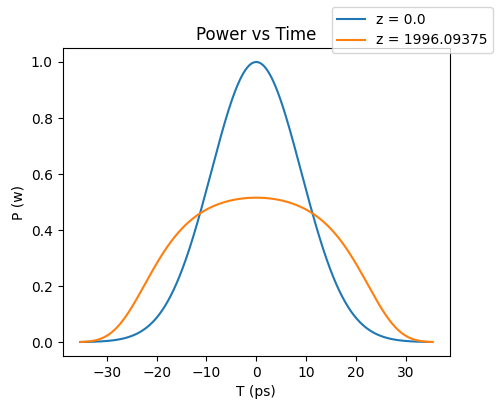
\includegraphics[width=\linewidth]{plots/plotPowerFL.png}
    \caption{}
    \label{trial1PowerFL}
\end{figure}

\begin{figure}%{i}{\linewidth}
    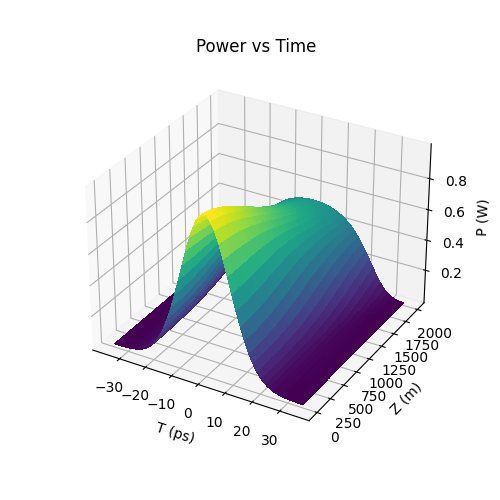
\includegraphics[width=\linewidth]{plots/plotPower3D.png}
    \caption{}
    \label{trial1Power3D}
\end{figure}

\begin{figure}%{i}{\linewidth}
    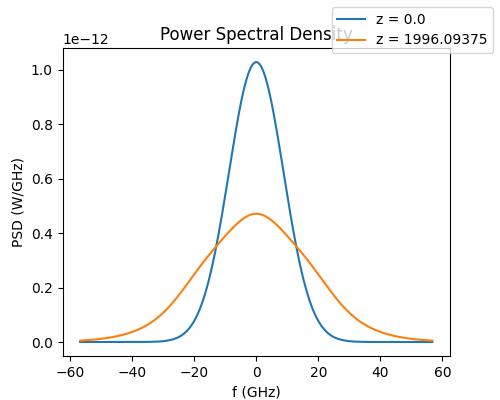
\includegraphics[width=\linewidth]{plots/plotFreqPFL.png}
    \caption{}
    \label{trial1FreqPFL}
\end{figure}

\begin{figure}%{i}{\linewidth}
    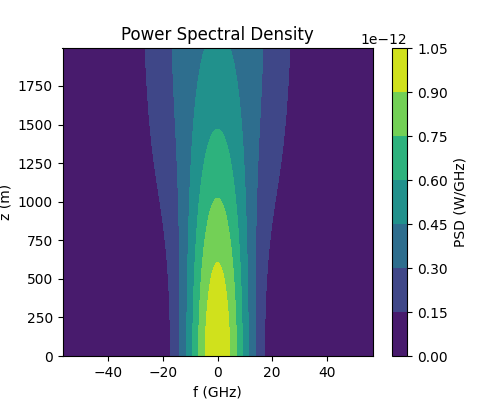
\includegraphics[width=\linewidth]{plots/plotFreqPFL2D.png}
    \caption{}
    \label{trial1FreqPFL2D}
\end{figure} 

\begin{figure}%{i}{\linewidth}
    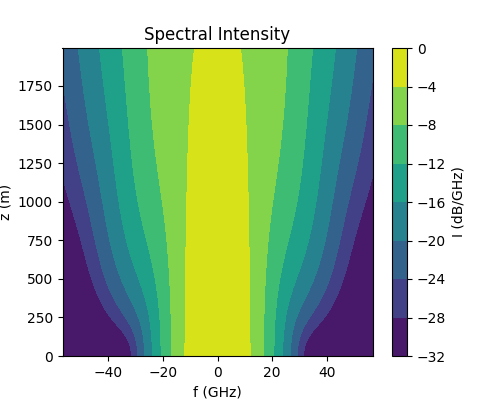
\includegraphics[width=\linewidth]{plots/plotFreqDbFL2D.png}
    \caption{}
    \label{trial1FreqDbFL2D}
\end{figure}

\begin{figure}
    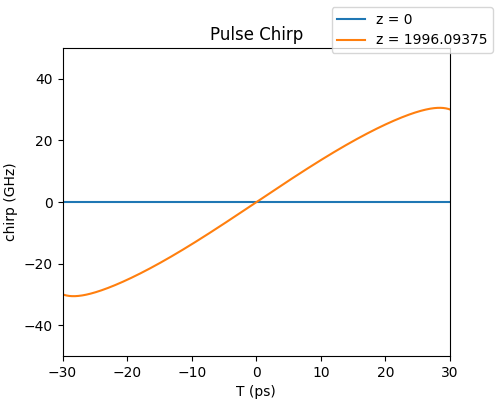
\includegraphics[width=\linewidth]{plots/plotChirpFL.png}
    \caption{}
    \label{trial1ChirpFL}
\end{figure}

Our results confirm our established intuitions. Group velocity dispersion is quantitatively visible, in both the power regime and spectral regime the power of the pulse with regard to the moving time frame $T$ and its frequency broadens, as shown in all figures [\ref{trial1PowerFL} \ref{trial1Power3D} \ref{trial1FreqPFL} \ref{trial1FreqPFL2D} \ref{trial1FreqDbFL2D} \ref{trial1ChirpFL}]
What is particularly interesting, and is most visible in the spectral analyses, is that the shape of the power spectral density loses its guassian shape as it tends to the end of the fiber. This is due to the effect of self phase modulation from the $\gamma$ parameter [\ref{trial1FreqPFL}], and shows that for a reasonably sized fiber this effect can have quite visible impact. Additionally, the effect of pulse chirping (the increase in the time dependency of its intantaneous frequency) is highly visible and symmetrical, as the structure and presence of 3rd order dispersion effects would predict.

\section{Solitary Waves / Solitons}
One interesting application of our simulation is the investigation of optical solitons. As for even standard fibers we can see the impacts of pulse broadening over short distances, engineers are interested in finding methods by which to preserve signal pulses for as long distances as possible. Keeping the amplitude of a signal sufficiently high can simply be done with amplifier components stored along a fiber, but this does not stop pulse broadening, which may lead to the overlapping of different wave packets and thus the destruction of transmitted data \cite{AgrawalChap3}. One solution to this problem starts with the initial pulse shape provided to the system. The nonlinear Schrodinger equation for optical fibers predicts the existence of optical solitons, or special pulses, that when configured correctly, employ a "cancelling out" effect between self-phase modulation and group velocity dispersion in order to create a pulse that self-sustains its shape as it propagates \cite{AgrawalChap5}. Solitons obviously do not stop the effects of loss, but are still quite useful in that they will not broaden to the extent that successive pulses may overlap. 

Our medium actually contains a space of differently ordered soliton solutions. Starting with the fundamental soliton, which is characterized by the integer order $N = 1$ \cite{Munaweera} 
$$u(0, T) = \frac{1}{\cosh(\tau)} e^{-iC\tau^2/2}$$
with $\tau$ being the normalized time reference frame $\tau = T/T_0$, and $C$ being an initial amount of "chirp" (phase shift) that does not contribute to the soliton behavior, so we may choose it to be any value, including $0$. After putting this into our simulation, with width $T_0 = 6.4 ps$, this time with a much higher dispersion level to elevate our confidence in the behavior of the soliton:
\begin{center}
\begin{tabular}{|c | c c|}
    \hline Parameter & Value & Units\\
    \hline
    $\beta_2$ & 20 & ps$^2$/km\\
    $\alpha$ & 0.2E-3 & dB/m\\
    $\gamma$ & 3E-3 & 1/W/m\\
    \hline
\end{tabular}
\end{center}
and propagating it for 1000 meters, our outputted graphs are quite intriguing.

\begin{figure}
    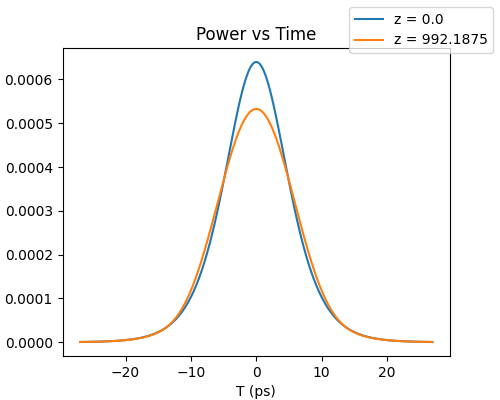
\includegraphics[width=\linewidth]{plots/sechPowerFL.png}
    \caption{}
    \label{sechPowerFL}
\end{figure}

\begin{figure}
    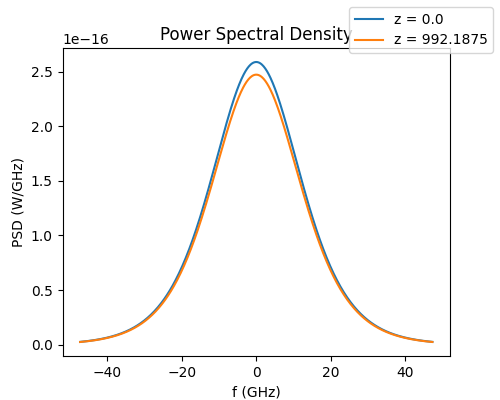
\includegraphics[width=\linewidth]{plots/sechFreqPFL.png}
    \caption{}
    \label{sechFreqPFL}
\end{figure}

\begin{figure}
    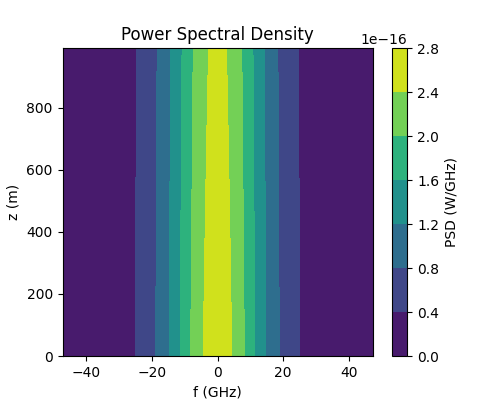
\includegraphics[width=\linewidth]{plots/sechFreqPFL2D.png}
    \caption{}
    \label{sechFreqPFL2D}
\end{figure} 

\begin{figure}
    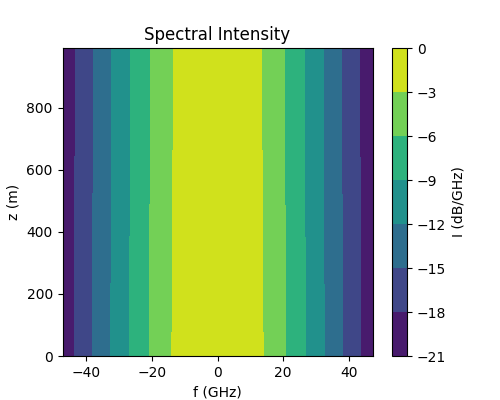
\includegraphics[width=\linewidth]{plots/sechFreqDbFL2D.png}
    \caption{}
    \label{sechFreqDbFL2D}
\end{figure}

\begin{figure}
    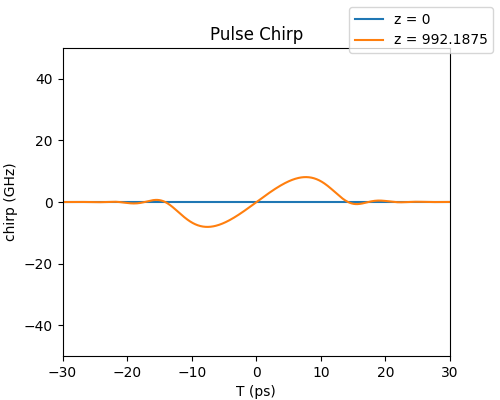
\includegraphics[width=\linewidth]{plots/sechChirpFL.png}
    \caption{}
    \label{sechChirpFL}
\end{figure}

Of particular interest is what has happened to the Power vs Time graph [\ref{sechPowerFL}]. It is quite clear that the overall pulse amplitude has decreased but it's overall spatial form is almost exactly intact. This is what we hope to see in the formation of an optical soliton. It is not entirely immune to pulse broadening, and any optical soliton wll break apart, as their form is attenuation dependent and their derivation is based on the assumption that changes in attenauative effects are relatively small \cite{AgrawalChap5}. There are higher order solitons ($N > 1$) as well, that maintain their pulse shape in an oscillatory manner, but these often rely on higher order dispersive effects that we have chosen to exclude from our simulation for the sake of simplicity.

Also note that the spectral power density [\ref{sechFreqPFL}] and spectral intensity [\ref{sechFreqDbFL2D}] has maintained a near perfect initial distribution, besides the loss effects and the increase in chirp apparent in [\ref{sechChirpFL}] This again demonstrates the partial cancellation of self phase modulation by the soliton, which has done the work of reinforcing its own frequency spectrum as it propagates.

\section{Dispersion Compensation}
Using solitons as a solution to the dispersion problem is limiting in that it places heavy constraints in the generation and shape of optical waves, and in most cases is very frequency dependent. In practice dispersion compensation is achieved through connecting anomalous and normal dispersive fibers such that the average dispersion on the pulse is reduced and thus the pulse broadening can be mitigated \cite{AgrawalChap5}. 

If we connect two fibers with different dispersive constants $\beta_{21}$ and $\beta_{22}$, each with lengths $L_1$ and $L_2$, we will find that the pulse evolution can be understood as a superposition of the dispersive effects in fourier space \cite{AgrawalChap5}:
\begin{align*}
    &A(L, T) = \mathbb{F}^{-1} \Bigl\{\\ &\tilde{U}(0, \omega) \mathrm{exp}(\frac{i}{2} \omega^2(\beta_{21}L_1 - \beta_{22}L_2) - i\omega t) \Bigl\}
\end{align*}
It is easy to see from here that the net dispersive parameter of this system will disappear when the term $\beta_{21}L_1 - \beta_{22}L_2 = 0$. This gives us a guide for selecting two fibers that will compensate the effects of dispersion. 

Let us investigate with our simulation once more, however this time we will get more exotic and introduce the condition that for $0 \leq z < 1000$, the fiber has dispersion parameter $\beta_2 = 20 ps^2/km$, and for $1000 \leq z < 1250$, the fiber has dispersive constant $\beta_2 = -80 ps^2/m$. This way, or condition to compensate for dispersion has been met. 

\begin{figure}
    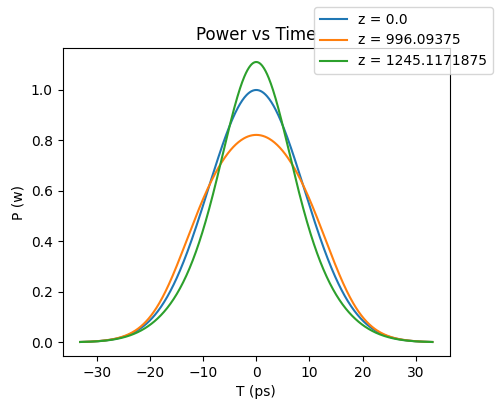
\includegraphics[width=\linewidth]{plots/compPowerFL.png}
    \caption{}
    \label{compPowerFL}
\end{figure}

\begin{figure}
    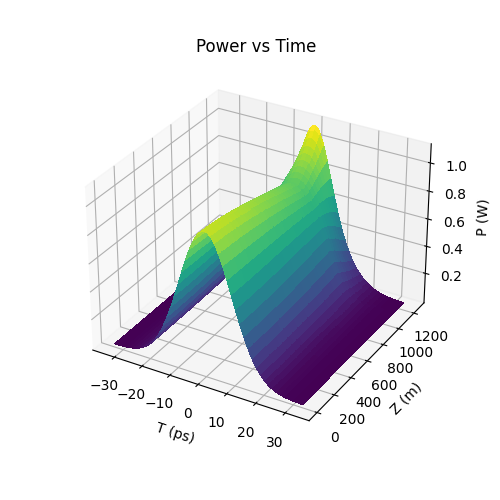
\includegraphics[width=\linewidth]{plots/compPower3D.png}
    \caption{}
    \label{compPower3D}
\end{figure}

\begin{figure}
    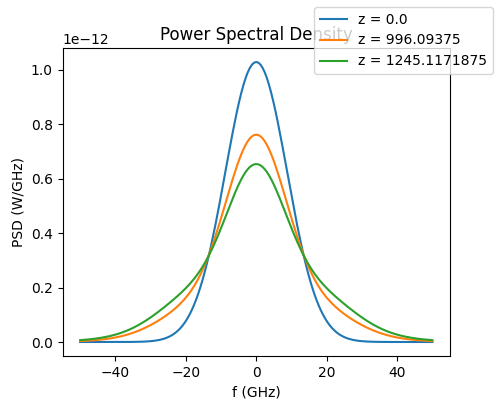
\includegraphics[width=\linewidth]{plots/compFreqPFL.png}
    \caption{}
    \label{compFreqPFL}
\end{figure}

\begin{figure}
    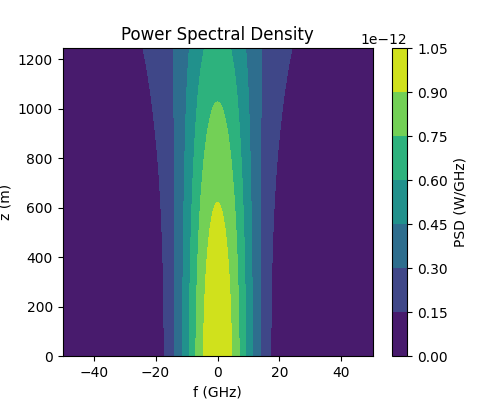
\includegraphics[width=\linewidth]{plots/compFreqPFL2D.png}
    \caption{}
    \label{compFreqPFL2D}
\end{figure} 

\begin{figure}
    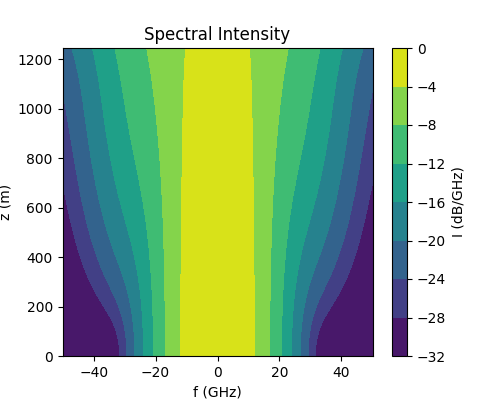
\includegraphics[width=\linewidth]{plots/compFreqDbFL2D.png}
    \caption{}
    \label{compFreqDbFL2D}
\end{figure}

\begin{figure}
    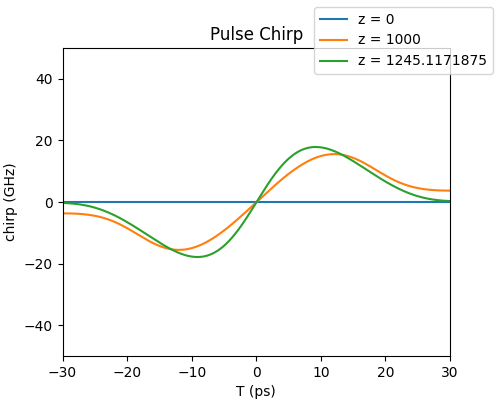
\includegraphics[width=\linewidth]{plots/compChirpFL.png}
    \caption{}
    \label{compChirpFL}
\end{figure}

Looking at the results of our simulation, it does seem that passing the pulse through the anomalous dispersion cable after it went through the normal dispersion cable had an impact on reducing the breadth of the Power vs Time graph [\ref{compPowerFL}], but in the spectral domain [\ref{compFreqPFL2D} \ref{compFreqDbFL2D}] the effects of self phase modulation are still highly visible and do not appear to be mitigated by this scheme.

The chirp [\ref{compChirpFL}] in this simulation increased constantly in both mediums, so if it is the desire of the engineer to de-chirp their signals as well, exploration of other methods (likely involving variable $\gamma$ term fibers) is required.

\section{Conclusion}
Though our simulation has demonstrated many interesting optical fiber cables of real world concern, these are only the most surface level investigations into the engineering of fiber communication systems and nonlinear optics as a whole. Much more sophisticated physical phenomenon such as Raman and Brillouin scattering and higher order polarization nonlinearities are worthy of their own discussion, and lead to fascinating and bizarre phenomenon such as birefringence (refraction dependent on light polarization), harmonic generation, and even cause certain cables to have no dispersion wavelengths which are optimal for centering guassian pulses around in order to minimize dispersion and phase modulation.

\section{Notes}
The code for this project can be found on \href{https://github.com/NConstantinides/PHYS273HProject}{Github}. Though no resources were explicitly taken from it, the split step fourier implementation by \href{https://www.youtube.com/@yourfavouriteta9282}{Your Favourite TA} on Youtube was of great help as a reference and his explanations of the processes made the project a much easier undertaking. His implementation can be found on \href{https://github.com/OleKrarup123/NLSE-vector-solver}{here} as well.

%----------------------------------------------------------------------------------------
%	BIBLIOGRAPHY
%----------------------------------------------------------------------------------------

\printbibliography[title={Bibliography}] % Print the bibliography, section title in curly brackets

%----------------------------------------------------------------------------------------

\end{document}
